\documentclass[conference]{IEEEtran}
\IEEEoverridecommandlockouts

\usepackage[british]{babel}
\usepackage[noadjust]{cite}
\usepackage{graphicx}
\usepackage[hyphens]{url}
\usepackage{paralist}
%\usepackage[pdftex,colorlinks=true,hyperfootnotes=false]{hyperref}

% reduce indent on all paralist environments
\setdefaultleftmargin{0.5cm}{}{}{}{}{}

\begin{document}

% paper title
\title{Smart Data-Harnessing for Financial Value in Short-Term Hire Electric Car Schemes}


% author names and affiliations
% use a multiple column layout for up to three different
% affiliations
\author{\IEEEauthorblockN{Peter Cooper\thanks{This work has been supported in part by Arup Group Ltd. through the Industrial Doctorate Centre in Systems at the University of Bristol.}}
\IEEEauthorblockA{Faculty of Engineering\\
University of Bristol\\
Bristol, UK\\
Email: peter.cooper@bristol.ac.uk}
\and
\IEEEauthorblockN{Tom Crick}
\IEEEauthorblockA{Department of Computing\\
Cardiff Metropolitan University\\
Cardiff, UK\\
Email: tcrick@cardiffmet.ac.uk}
\and
\IEEEauthorblockN{Theo Tryfonas}
\IEEEauthorblockA{Faculty of Engineering\\
University of Bristol\\
Bristol, UK\\
Email: theo.tryfonas@bristol.ac.uk}}

% conference papers do not typically use \thanks and this command
% is locked out in conference mode. If really needed, such as for
% the acknowledgment of grants, issue a \IEEEoverridecommandlockouts
% after \documentclass

% use for special paper notices
%\IEEEspecialpapernotice{(Invited Paper)}

% make the title area
\maketitle


\begin{abstract}
In the developed world, two distinct trends are emerging to shake-up
the current dominance of privately-owned, combustion motor car
transport. The first is the emergence of the electric powertrain for
vehicles as an affordable and mass-marketed means of transport. This
carries with it the potential to address many of the immediate
shortcomings of the current paradigm, especially CO2 emissions, air
and noise pollution. The second is the rise of new hire models of car
ownership -- the concept of paying for the use of a car as and when
you need it. This carries with it the potential to address many of the
existing issues: outlay-induced car use, residential parking and
social division.  On a similar timescale, we are witnessing the rise
of smart technologies and smart cities, concepts that use data about
the state of a system or elements of it to create value.

There have been relatively few examples of schemes that have combined
the electric and hire-model concepts, despite the huge potential for
synergy. Indeed, the majority is against them on both counts -- cars
are predominantly privately-owned and driven by internal combustion
engines. Nevertheless, there is significant potential for this to
change over the coming years.
\end{abstract}

% For peer review papers, you can put extra information on the cover
% page as needed:
% \ifCLASSOPTIONpeerreview
% \begin{center} \bfseries Keywords \end{center}
% \fi
%
% For peerreview papers, this IEEEtran command inserts a page break and
% creates the second title. It will be ignored for other modes.
%\IEEEpeerreviewmaketitle

\begin{IEEEkeywords}
Electric Vehicles, Vehicle Hire Models, Smart Technologies, Smart
Monitoring, Smart Cities, Big Data, Environmental Impact
\end{IEEEkeywords}

\section{Introduction}

The last decade has demonstrated the current Western private transport
paradigm has a finite lifespan; a transport culture that consists of
overwhelmingly privately-owned internal combustion engine automobiles
is unlikely to survive the next 50 years.

Two distinct cultural trends are bringing about its demise. Most
notably is the emergence of electrical motors as the primary alternate
fuel source in powertrains for automobiles. Almost all of the world's
major automotive companies have released purpose-designed electric
cars; some have had made strategic investment in the concept as to
release an entire electric car range, underpinned by efficient driving
technologies, for example BMW's i Series and EfficientDynamics
system\footnote{\url{http://www.bmw.co.uk/en_GB/topics/discover-bmw/efficientdynamics/technologies.html}}.
The direct environmental benefits of electric cars, lower particulate
emissions, lower noise emissions and the potential for lower CO2
emissions, are highly significant. Legislation in many countries is
acting in two ways: penalising internal combustion engine users, and
incentivising the purchase of EVs. Electric cars bring with them
several caveats, however: the capital cost of EVs, predominantly due
to current battery technology, is yet to be comparable to an
equivalent internal combustion engine car; the embodied carbon of EVs,
again due to the battery component, is on average considerably higher
than an equivalent internal combustion engine, and the generation of
electricity to meet charging patterns brings with it considerable
logistical difficulties.

More in its infancy is the trend of transitions in car use models. In
other modes of private transport, predominantly bike use, an
increasing number of users are opting to participate in short term
hire models of use, particularly in urban contexts. Rather than baring
the capital and logistical cost of owning a bike, individuals hire the
bike for a nominal fee from a given node near their origin, complete
their journey, and return the bike to a node near their
destination. Once seen as radical, examples such as London's cycle
hire (``Boris Bike'')
scheme\footnote{\url{http://www.tfl.gov.uk/modes/cycling/barclays-cycle-hire}}
demonstrated not only the feasibility of the business model, but also
the efficacy of the indirect benefits, illustrated by significant
increase in cycling in the city.

A third, more generalised trend in societal organisation is the
emergence of the smart city theorem. This capitalises on the use of
`smart technologies', systems that harness opportunities data presents
to provide value; in the smart city theorem this cuts across city
system boundaries. In other words, the data from one particular
aspect, such as waste disposal, not only informs the operation of
waste disposal, but also, for example, influences how the road system
operates during waste collection hours.

However, transition is, at present, slow. Electric cars only make up a
negligible share of the UK car market (with limited infrastructure
outside of major urban areas), short-term hire transport models have
yet to be proved beyond simpler transport situations, such as
bicycles, and smart cities are, in many cases, little more than a long
term strategic aspiration, with some instances of demonstrators, most
of which are too early in their lifetime to be able to provide any
real conclusions.

The actions of policy makers in the next 10 years will dictate
how much these trends are harnessed, encouraged or ignored, and
ultimately how the UK's transport culture changes as a result.

\section{UK Policy Context}

Politically, the UK's transport strategy lacks resolve and strategic
planning. A heavily departmentalised, part-privatised transport system
lacks consistent objectives, agendas or priorities. Multimodal travel
design is attempted coarsely, with new transport systems being
overlaid on the old, with little foresight or retrospective
adjustment.

Over the last 60 years, transport journey makeup has transitioned
rapidly from public transport-dominated to a private
transport-dominated network, stabilising at the end of the 2010
decade. Vocal, anti-automotive political agendas, global recession and
rising oil prices have all emerged since as powerful, anti-private
transport influences. However, they have done little to reduce private
transport, with transport behaviours appear largely unchanged, tending
instead to a marginally lower equilibrium level today. This is
displayed in Figure~\ref{fig:uktransportshare}, contextualised by the
historical car ownership trends (cars per person in the UK): 0.004
(1909), 0.08 (1950) and 0.55 (2012).

% and the corresponding car ownership trends in
% Figure~\ref{fig:ukcarsperperson}.

\begin{figure}[!htp]
\centering
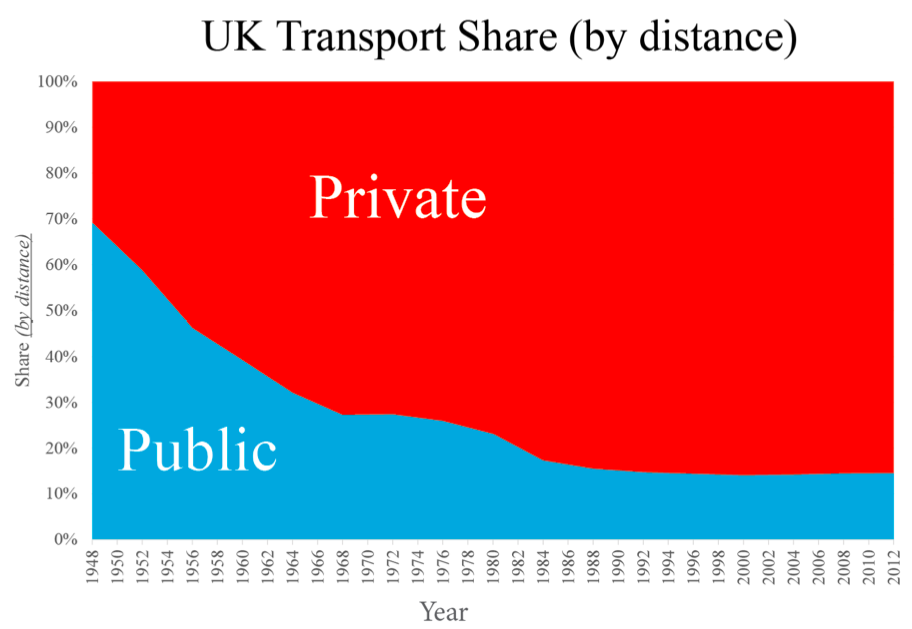
\includegraphics[width=\columnwidth]{images/uktransportshare.png}
\caption{Car ownership trends in the UK}
\label{fig:uktransportshare}
\end{figure}

% \begin{figure}[!htp]
% \centering
% 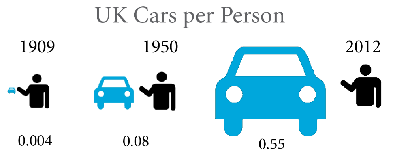
\includegraphics[width=\columnwidth]{images/ukcarsperperson.png}
% \caption{Transport share in the UK}
% \label{fig:ukcarsperperson}
% \end{figure}

In theory, it is clear that public transport is both technically (in
terms of emissions per head) and systematically (second-order effects,
such as congestion, social and economic consequences) superior to
private transport. However, it is equally apparent that the unit cost
of converting a percentage of transport users from private to public
transport increases with conversion. For example, to convert the
easiest first 10\% of users, a network of urban buses and trains can
be run cost-effectively and efficiently. The last 10\% of the
population, however, requires a vast and complex network that operates
constantly and at high frequencies, and is for all intents and
purposes, impossible to deliver. As such, it is clear that there is a
fraction of transport that, for reasons of financial and practical
limitations, will always remain private transport, and that that
fraction is not necessarily `small'. Although the UK does not
currently operate at or even near this `minimum' private transport
threshold, acknowledgement that any such unavoidable level exists is
not popular politically.

As such, in private transport, there is an idea that any impacts, both
technically and systematically, should be mitigated. This is a popular
and high-growth area of research; within the last 20 years, personal
automobile efficiency has improved drastically. Today, alternate
powertrains such as electric motors, more efficient and less polluting
that internal combustion engines, are not only technically viable, but
a key component of many automotive giant’s strategies; the
aforementioned BMW i Series range is a high profile example of
significant strategic investment in the transition of retail
automobiles to EVs. However, it is clear that drivetrain transitions
alone cannot deal with the systematic drawbacks of private transport,
such as congestion, special requirements of parking and social
isolation of the have-cars and have-nots. Technological suggestions
for these problems do exist, such as driverless, automated cars and
personal rapid transit (PRT) schemes, but both are a long way from a
ready-to-rollout status. Crucially, for every change that improves the
negative impact of private transport, or more accurately, convincingly
depicts itself as doing so, private transport is further legitimised,
and efforts to transfer journeys to public transport are weakened.

Political action is thus limited by this simple catch-22: public
transport is the ideal, but impractical to reach saturation. Private
transport is undesirable, but unavoidable, yet efforts to improve it
also make it more prevalent. Mathematically, you might argue there
thus exists an optimum -- a level of improvement of private transport
that, when the reduction in public transport uptake is factored in,
results in the lowest overall impact in the UK's travel
emissions. Whether or not this thought experiment is a fair
simplification, there is a more logical and pragmatic answer -- that
transport strategy should be considered on a holistic level, and the
interaction between private and public transport held as
crucial. There are many more secondary effects that could also be
considered from this first deduction; not all improvements to private
transport reduce public transport uptake to the same degree; nor is
the UK a homogenous mass of two types of transport user. Attempts to
penalise private transporters who could transfer to public transport
and do not, such as through taxation, frequently damages those who
cannot transfer.

Ignorance to these wider socio-cultural relationships, brought about
by the private/public segmentation of both traditional transport
strategies and the segmentation of organisations tasked with dealing
with each, allows these undesirable, unintended consequences to
continue and prevent technological and political progress.

\subsection{Electric Vehicles}

Electric vehicles (EVs) can offer an environmentally sustainable
alternative to internal combustion engines (ICEs). EVs are powered by
a battery which is charged through the electricity network. Alongside
reducing carbon emissions, EVs can also improve noise and air quality,
provide savings for consumers and reduce dependency on specific fossil
fuels~\cite{postevs:2010}. It is widely accepted that an alternate
energy source is necessary for the UK transport network in the near
future, and electrification is currently considered the most likely
choice.  The Department for Transport (DfT) predicts that by 2020
there will be 1.5m EVs on the road in the UK~\cite{dft:2008}.

There are a number of barriers to the adoption of EVs. Many of these
are psychological, for example range anxiety; consumers worry that
they may `run out of juice'~\cite{oflev:2011}. However, 95\% of all
vehicle journeys in the UK are less than 25 miles
(40km)~\cite{oflev:2011}, only a small proportion of existing EV's
range. Other consumer barriers include: concerns over battery
lifetimes, the risk associated with investing in a relatively new
technology and the current, comparatively large capital investment
required to purchase an EV.

Personal vehicles and small commercial vehicles account for 13\% of
all UK carbon emissions~\cite{lumsden:2012}; by transitioning to EVs
in these sectors, the overall volume of emissions could be
significantly reduced.  Due to the nature of UK car culture, fleet
vehicles accounted for 63\% of all new vehicle sales in the UK in 2011
and as such are a dominant influence on the type of cars for sale in
the used market~\cite{fleets:2012}. There is a growing trend for EVs
in fleet vehicles, so it is likely a tangible used EV market will
start to emerge in the next five years.

Electrified public transport is still a fairly new area of
interest. Hybrid buses have been introduced in a number of cities to
reduce emissions, with London having 368 hybrid diesel-electric buses
in operation in 2014~\cite{tfl:2009}. In January 2014, the first
inductive charging all-electric buses were introduced into
service in Milton
Keynes\footnote{\url{http://m.bbc.co.uk/news/technology-25621426}}. The
UK Government is supporting investment in low carbon bus technology
through the Green Bus
Fund\footnote{\url{https://www.gov.uk/government/publications/details-of-the-green-bus-fund}},
as well as many other general, sustainability-targeted funding
packages.

\subsection{Smart Technologies}

Smart technology is a new and rapidly growing concept; as such, a
consensus of its exact definition has yet to be reached. However,
interviewed academics~\cite{elecgen:2013}, industrial
experts~\cite{buscher:2014} and a number of
papers~\cite{komninos:2002,arup-et-al:2011,harrison+abbottdonnelly:2011,batty-et-al:2012}
identify the fundamental, unifying theme as the use of data. The rise
of interest in data-based possibilities for the built environment has
been fuelled by three key developments:

\begin{compactenum}
\item {\textbf{The rapid increase in the production of data.}}
  Computer scientists have stated that many social trends, such as the
  rise of Internet connectivity (specifically high-speed mobile
  Internet), and social networking, has caused an exponential
  increase in the production of data. Today, almost 30 petabytes of
  data exists on Facebook alone\footnote{\url{http://www.theguardian.com/news/datablog/2014/feb/04/facebook-in-numbers-statistics}}. The abundance of such a
  resource has spurred consideration as to its potential use.
\item {\textbf{The rapid increase in the ability to collect specific
      data.}} Improvements in sensor and communication technology have
  meant the installation of data collection devices is now both financially and
  spatially practical. The development of mesh networks, the notion of deploying equally
  spaced sensors across a large area to give a high resolution of data
  or the ability to track the movement of entities. Furthermore, the
  Internet of Things, the notion that with the deployment of
  connected sensors on existing everyday objects, interactions that
  are currently machine-human-machine could simply be machine-machine,
  allowing many such processes to be faster, cheaper and  more
  convenient. 
\item {\textbf{Improvements in data storage and processing.}} Following
  Moore’s Law/Kryder's Law, storage is far cheaper than ever before, allowing
  this vast data to be stored. Processing power is also much greater,
  allowing complex trends from data on scales so vast as a city to be
  processed and actioned fast enough to be considered `live'.
\end{compactenum}

Many such sources refer to data as a raw material (perhaps even an
emerging `utility', joining electricity, gas, water and telephone
networks), creating the notion that data can and should be used as an
input to a business model that is then translated to value. In recent
years the practicalities of collecting and processing a vast quantity
of high value data of a system, as discussed, has developed
significantly~\cite{arup-et-al:2011}. Such a system could be a house,
business or city, with data being the movement of containers in a
factory, the journeys of cars across an urban network, or the use of
electricity residentially. The sheer volume of data available for such
a large range of systems has led to the term `big data’, now commonly
used to refer to a datastream large enough to make smart technologies
feasible~\cite{hollands:2008,ibmsmartcities:2009,ciscoconcities:2010}.

Smart technologies are usually defined as microsystems within these
larger systems that carry out an action based on the collected
data. Smart technologies are typically based on an existing action
that, it is theorised, could be completed more effectively -- as well
as sustainably~\cite{cosgrave-et-al:2014} -- with the assistance of
data~\cite{arup-et-al:2011}. More effectively can be interpreted as:

\begin{itemize}
\item {\textbf{Faster:}} such as using traffic distribution to update
  signs in real time, rather than the slow, reactive methods
  by which traffic is informally advised against taking certain
  routes.
\item {\textbf{Fairer:}} such as smart pricing for grid electricity,
  whereby data on the national grid is used to charge those who
  use electricity when demand is highest (when the cost of generation
  is highest), a cost that is reflective of the cost to supply the
  electricity to them. 
\item {\textbf{At lower cost:}} whereby flow sensors in water pipes
  can be used to deduce the exact location of leaks when they emerge,
  rather than expensive and time-consuming visual inspections.
\item {\textbf{Without human interaction:}} whereby more interactions
  can be machine-machine rather than using a human intermediary, such
  as when an inspection robot is automatically sent to the site of a
  machine malfunction in a factory, rather than a human noticing the
  fault and piloting the robot manually. This can improve instances of
  both human error, hesitation and subjective judgment (for better or
  for worse). 
\end{itemize}

Smart cities are urban areas in which smart technologies are taken a
step further, and different city sub-systems such as waste disposal
and water provision are integrated. In practice, this results in smart
technologies using data streams from neighbouring
systems~\cite{shapiro:2006}. For example, in a theoretical world where
there is near saturation of EVs, preemptive car journey data could be
used to adjust the national grid's generation so as to ensure the
correct amount of power is generated for the EVs recharging at the
time they are expected home. Such intelligence allows for more
efficient generation, avoiding the short-notice generation that is
currently employed~\cite{tsoukalas:2008}.

\section{The Role of Smart Technology}

\subsection{Approach}

We will now consider the role of smart technology within the future’s
transport strategy, specifically integrated private/public and
electric transport solutions for a range of suggested concepts in
existing literature covering smart technologies of a number of
different industries, we will consider the nature and operation of
each in the wider smart transport context.

% Throughout this exploration, an appropriate valuation method will be
% chosen depending on the nature of the technology in question. For each
% example we will speculate the first year value of the technology,
% commenting on the total lifetime value later on.

For the purposes of this study we will consider the benefits of these
smart technologies specifically from a private sector business case
viewpoint; that is to say, primarily the financial and economic
benefit they could bring (although they also have significant social,
political and environmental benefits).

\subsection{Cars}

Standard car hire industry practice is to operate a maintenance regime
that involves inspection above the recommended frequency, designed to
reduce the time between inspections when the car may suffer from a
freak failure. Freak failures are defined as those whereby there was
no indication at the last inspection that the car would fail before
the next testing.

Using health and usage monitoring sensors attached to key components
in the car, the car hire operators can get an understanding of level
of car mechanical state close to that offered by an inspection, but
constantly and in real time. This could drastically reduce the rate of
freak failures and, if the sensor coverage was sufficient enough,
potentially allow reductions in human servicing.  This concept is
already well understood in industrial contexts and frequently
realised. The value from this system comes from improved reliability
and efficiency of the car hire service.


\subsection{Live Air Quality Management}

Bristol (a major city in the west of England) monitors air quality by
semi-permanent installations at specific areas around the city.  In a
typical UK urban environment, particularly one with no major industry,
air quality is primarily determined by road transport emissions.  As
such, if it was possible to understand the overall distribution of
vehicles in the city at any one point in time, it would be possible to
estimate, with relative accuracy, the air quality throughout the
entire city. At present, in some areas of the city, car flow is
monitored by car-recognising cameras. These however are sparse and
expensive to install.

The car hire EVs are likely to use the same roads to the same
intensity of other cars on the road at that time. In other words,
their road routing behaviour is likely to be very similar, if not
identical, to the rest of the cars on the road at that time. As such,
a critical resolution of hire cars is necessary to deduce an estimate
of the wider car resolution. We will examine critical resolutions in
detail at the end of this section.  The value from this system comes
from the created market of vending car locational data to Bristol City
Council.

% \begin{figure}[!htp]
% \centering
% 
\includegraphics[width=\columnwidth]{images/dontchokebristol.png}
% 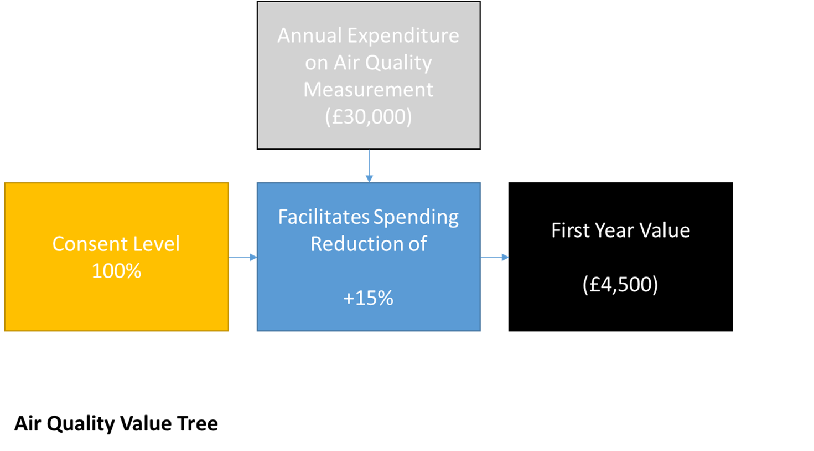
\includegraphics[width=\columnwidth]{images/airqualityvt.png}
% \caption{Air quality value tree}
% \label{fig:airqualityvt}
% \end{figure}

\subsection{Live Accident Reporting}

Similar to in-car monitoring for maintenance, vehicles can also be
fitted with impact sensors, altering the car hire management that a
car has suffered a serious crash, allowing them to contact the
authorities.  Due to the significant improvement in road safety
regulations, mobile phones have already improved road transport since
the mid-2000s, and the relative rarity of isolated crashes, it is
unlikely the value case here can be made from a practical improvement
in fatality rates from car hire use.

Instead, it is probable that the main benefit of such a system would
be perceptual – improved piece of mind for the customer that a system
will be in place to constantly evaluate their safety.  However, the
increase in service from such a technology yields a relatively
insignificant revenue stream.

\subsection{User Journey Data}

One of the fastest growing applications of data is within retail and
leisure industries.  Many organisations using big data have shown that
advertisement conversion rates (the percentage of individuals who act
on an advertisement they have seen) can be greatly increased by
accurate targeting of the advert to the correct
recipient. Traditionally, this would be done by geographical area or
age group. More recently however, with the ability to better express
to the world your other preferences and personal situation through
social media networks, it is possible to advertise to people of a
specific relationship status, group affiliation or fans of similar
services. Facebook and Spotify are prime examples of how specific
demographic, geographic and chronological conditions are set to not
only able to return high conversion rates, and thus, expensive
advertising to customers, but also, as a result, able to vend smaller
advertising exposures as a tangible product. This means a greater
number of clients, and thus a more robust business model.

In the car hire, two potential avenues of value creation are possible.
Firstly, information on the journeys of car hire individuals alongside
the time they drive and their personal characteristics, could be
vended in a data package to companies in retail and leisure
industries. These companies would have otherwise had to undertake
expensive customer research, thus the value is clear. However, this is
very likely to suffer from extremely low consent rates, as it would
perhaps be the most invasive form of personal data harvesting
currently in existence. Alternatively, consent rates may well be much
higher if the data was instead used to form targeted advertising at
point of booking. This way, organisations could offer discounts to
individuals it feels it may be able to convert to using their business
on the trip, incentivising them to consent to the scheme. Furthermore,
this could be done dynamically through the common advanced display
systems that are available in modern automobiles. The revenue stream
here will be two fold: the advertising organisations will pay for the
in-car advertising rights, and individuals would be more inclined to
travel through the hire car if special offers would be available.  The
primary value from this system comes from the vending of targeted,
data-based advertising of in-car and pre-booking advertisement to
local businesses.


\subsection{Smart Pricing Congestion Control}

An alternate method to control congestion is to bring economic forces
to bare on when an individual chooses to travel. In practice, the car
hire smart pricing would include an additional influence based on the
expected congestion of the roads at point of travel, attempting to
deter travel that would exacerbate the congestion.  Ultimately, this
requires the highest critical resolution of hire cars of all the smart
technologies addressed here, by some margin, perhaps at least
25\%. Furthermore, many ethical dilemmas exist. If the resolution is
lower than 50\%, it might be extremely unpopular that the most
sustainable cars are essentially `taxed' into staying off the roads,
while the unsustainable private transport is free to do as it
wishes. Although such a pricing technique would not be unlike current
train pricing structures, the freedom to use a car when one desires is
heavily ingrained in Western society, and it's likely any such pricing
on that logic would need to be mild.


\subsection{Charging Habits}

Similar to the understanding of how individuals operate electric cars,
the UK's National Grid\footnote{\url{http://www.nationalgrid.com/uk/}}
would be interested in how individuals charge their EVs, as this will
heavily influence how the grid develops in the next 50 years.
Although typically our EV's have predetermined charging patterns, EVs
that are taken on multi-day rentals will most likely require charging
to address the specific needs of the hirer. This provides a valid
insight into the charging habits of EV users. The value from this
system comes from the created market of vending charging habits to the
UK's National Grid.


\subsection{Car Positional Data}

One of the issues with an electric car hire scheme, as discussed
previously, is the increased layover time incurred by charging. This
has been shown to be manageable in its standard incarnation, but
certain instances could exacerbate this weakness, or simply be a
problem for car hire management schemes in general. For example the
following situations within a booking could threaten the ability to
service later bookings:

\begin{compactenum}
\item {\textbf{Inclement driving conditions:}} EVs are susceptible to
  have sizeable variation of energy use per mile depending on driving
  conditions. Cold weather can have negative effects on electric
  torque. Additionally, heaters in EVs are unable to use the waste
  heat that a combustion car generates, so additional power from the
  battery is required; as much as 15\% in certain
  circumstances~\cite{postevs:2010}. Live
  battery data can allow the car hire management system to know the
  exact power use of a journey.
\item {\textbf{Congestion:}} Traffic can significantly decrease the
  efficiency of the EV; although the effect is lessened when compared
  to a combustion car as EV engine can turn off and on
  seamlessly. More significantly, congestion greatly increases the
  journey time. Car speed data and GPS location data can inform the
  booking management system when a car is stuck in traffic.
\item {\textbf{Satellite navigation:}} If an individual decides to take a longer
  route home, or even a route of the same duration of time but a
  greater use of charge (such as a longer motorway route compared to a
  slower trunk route). Live satellite navigation data can inform the booking
  management system the minute the drive has this intention. 
\end{compactenum}

Pre-warning of any of these unforeseen circumstances can allow
immediate shifting of the booking system to reflect increased hire
duration or increased charging duration. This will prevent people
booking in a time when the car will now be driving/charging. The value
from this system comes from improved reliability of the car hire
service.

\subsection{Barriers and Enablers}

Each of these data streams and their associated benefits require
capital and operational expenditure to put in place the infrastructure
and staff that would facilitate the systems. Even without estimating
this, it can be seen that a number of technologies are immediately
unable to be financially viable, at least in isolation. Needless to
say, this theoretical value is not instantly realisable. Considerable
barriers exist to not only the creation of the value, but also the
smart technologies themselves. At present legislation in the UK around
renewables and EVs is under general scrutiny and review. Feed-in
Tariffs (FITs) and other payouts for balancing services are
complicated and have questionable longevity and there is little
governmental impetus in the UK for smart pricing on a balancing
level. Considerable psychological inertia also exists in some
businesses as to the idea of data as a source of value.  The issue of
critical resolution is also present --
Figure~\ref{fig:bristolcardensity} demonstrates varying accuracy from
predicting traffic levels at different sensor penetration.


\begin{figure}[!htp]
\centering
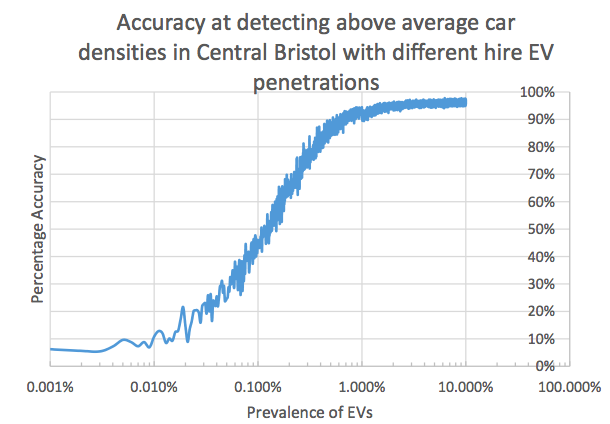
\includegraphics[width=\columnwidth]{images/bristolcardensity.png}
\caption{MATLAB modelling of the accuracy of extrapolating to find
  congestion from EV cars in Bristol, UK}
\label{fig:bristolcardensity}
\end{figure}


\section{Conclusions} 

\begin{figure}[!htp]
\centering
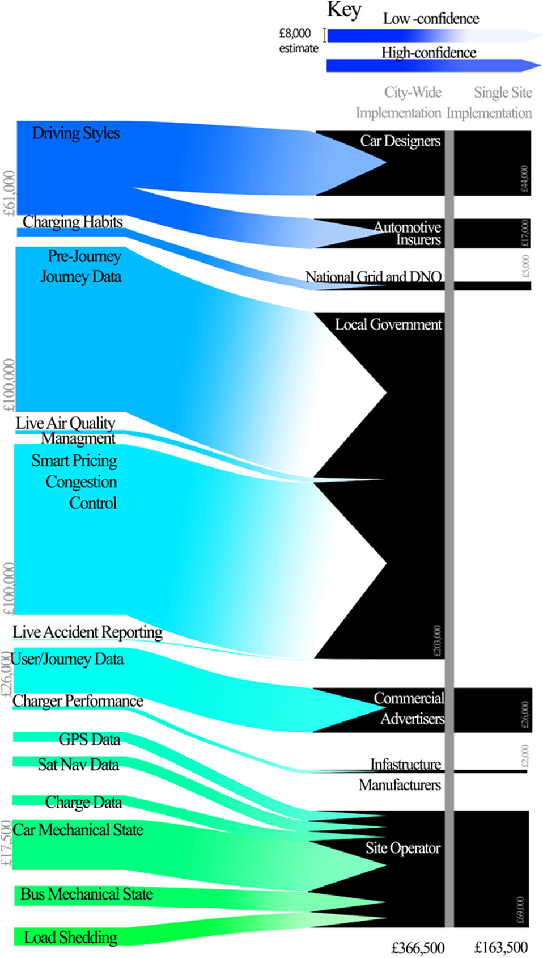
\includegraphics[width=\columnwidth]{images/sankey.png}
\caption{A Sankey diagram of the data value and confidence, along with
  single site vs. multisite implementations}
\label{fig:sankey}
\end{figure}

It is clear there is great variation in the nature and quantity of
value in smart technologies with short term EV hire. These are
presented in Figure~\ref{fig:sankey}. As a general rule, there are
three categories: 

\begin{compactitem}
\item Firstly, those that have the greatest benefit but are also the
  most speculative, having the highest critical masses and requiring
  the greatest stakeholder buy-in. However, their benefit is
  extreme. These also have the highest quantity of non-financial
  benefit, typically environmental, which is often equivalent to, or
  in some cases higher, than the economic and financial benefits. These
  are typified by the smart pricing congestion control and the dynamic
  traffic routing. Although there is little probability that this
  group will be implemented in the near future, the significant potential
  cannot be ignored, and would serve well as a long term agenda for
  local council, be it with implementation through a smart transport hub or
  elsewhere.
\item Secondly, a middle group, with moderate benefit whose
  speculation is somewhat less, but typically relies on a small, niche
  market for vending, and as such hinges significantly on this for any
  value at all. Driving styles is a typical examples of this. While
  there is some variation in the group -- spin off elements such as the
  journey data, advertising approach fairs much better -- it is
  difficult to label these as a quality. How UK law changes with respect
  to data use, as well as how contract culture changes with respect to
  data transactions will have a great influence. Many local
  governments or devolved city regions, including Bristol, are
  aspiring to wider open data initiatives, a
  system where similar data sets are freely available (and reusable),
  and the data is realised through the new businesses that open as a result. This
  stands, at least in some lights, in contrast to this category's
  technologies. 
\item Thirdly, and bucking the trend, is a group with moderate
  benefit, but whose speculation is low and requires only internal
  participation. This third group, typified by the smart pricing and
  car component monitoring, stand out as having the greatest
  appeal. 
\end{compactitem}

Ultimately, there is considerable potential for smart technologies to
transform not only the profitability of short term EV hire schemes,
but the wider societal benefit of the concept. Which of the above
segments are most appropriate to focus on will depend on the exact
context and buy-in from external stakeholders. It is equally apparent,
however, that the world has some considerable catching up to do --
socio-culturally, legislatively and psychologically -- if any of these
concepts are to be easily implemented, let alone the concept of the
short-term EV and its benefits thriving across the globe.


%\newpage

% trigger a \newpage just before the given reference
% number - used to balance the columns on the last page
% adjust value as needed - may need to be readjusted if
% the document is modified later
%\IEEEtriggeratref{28}
% The "triggered" command can be changed if desired:
%\IEEEtriggercmd{\enlargethispage{-5in}}

% references section
\bibliographystyle{IEEEtran}
\bibliography{sose2015}

% that's all folks
\end{document}


